\section{User Interface}
Based on the website prototypes in \secref{sec:prototype}, a user interface is implemented.
As can be seen from the prototype, the website has many windows, so only the some essential ones are shown.
The first we look at is the start page, which can be seen in \figref{fig:UI-overview}.

\begin{figure}[h]
	\centering
	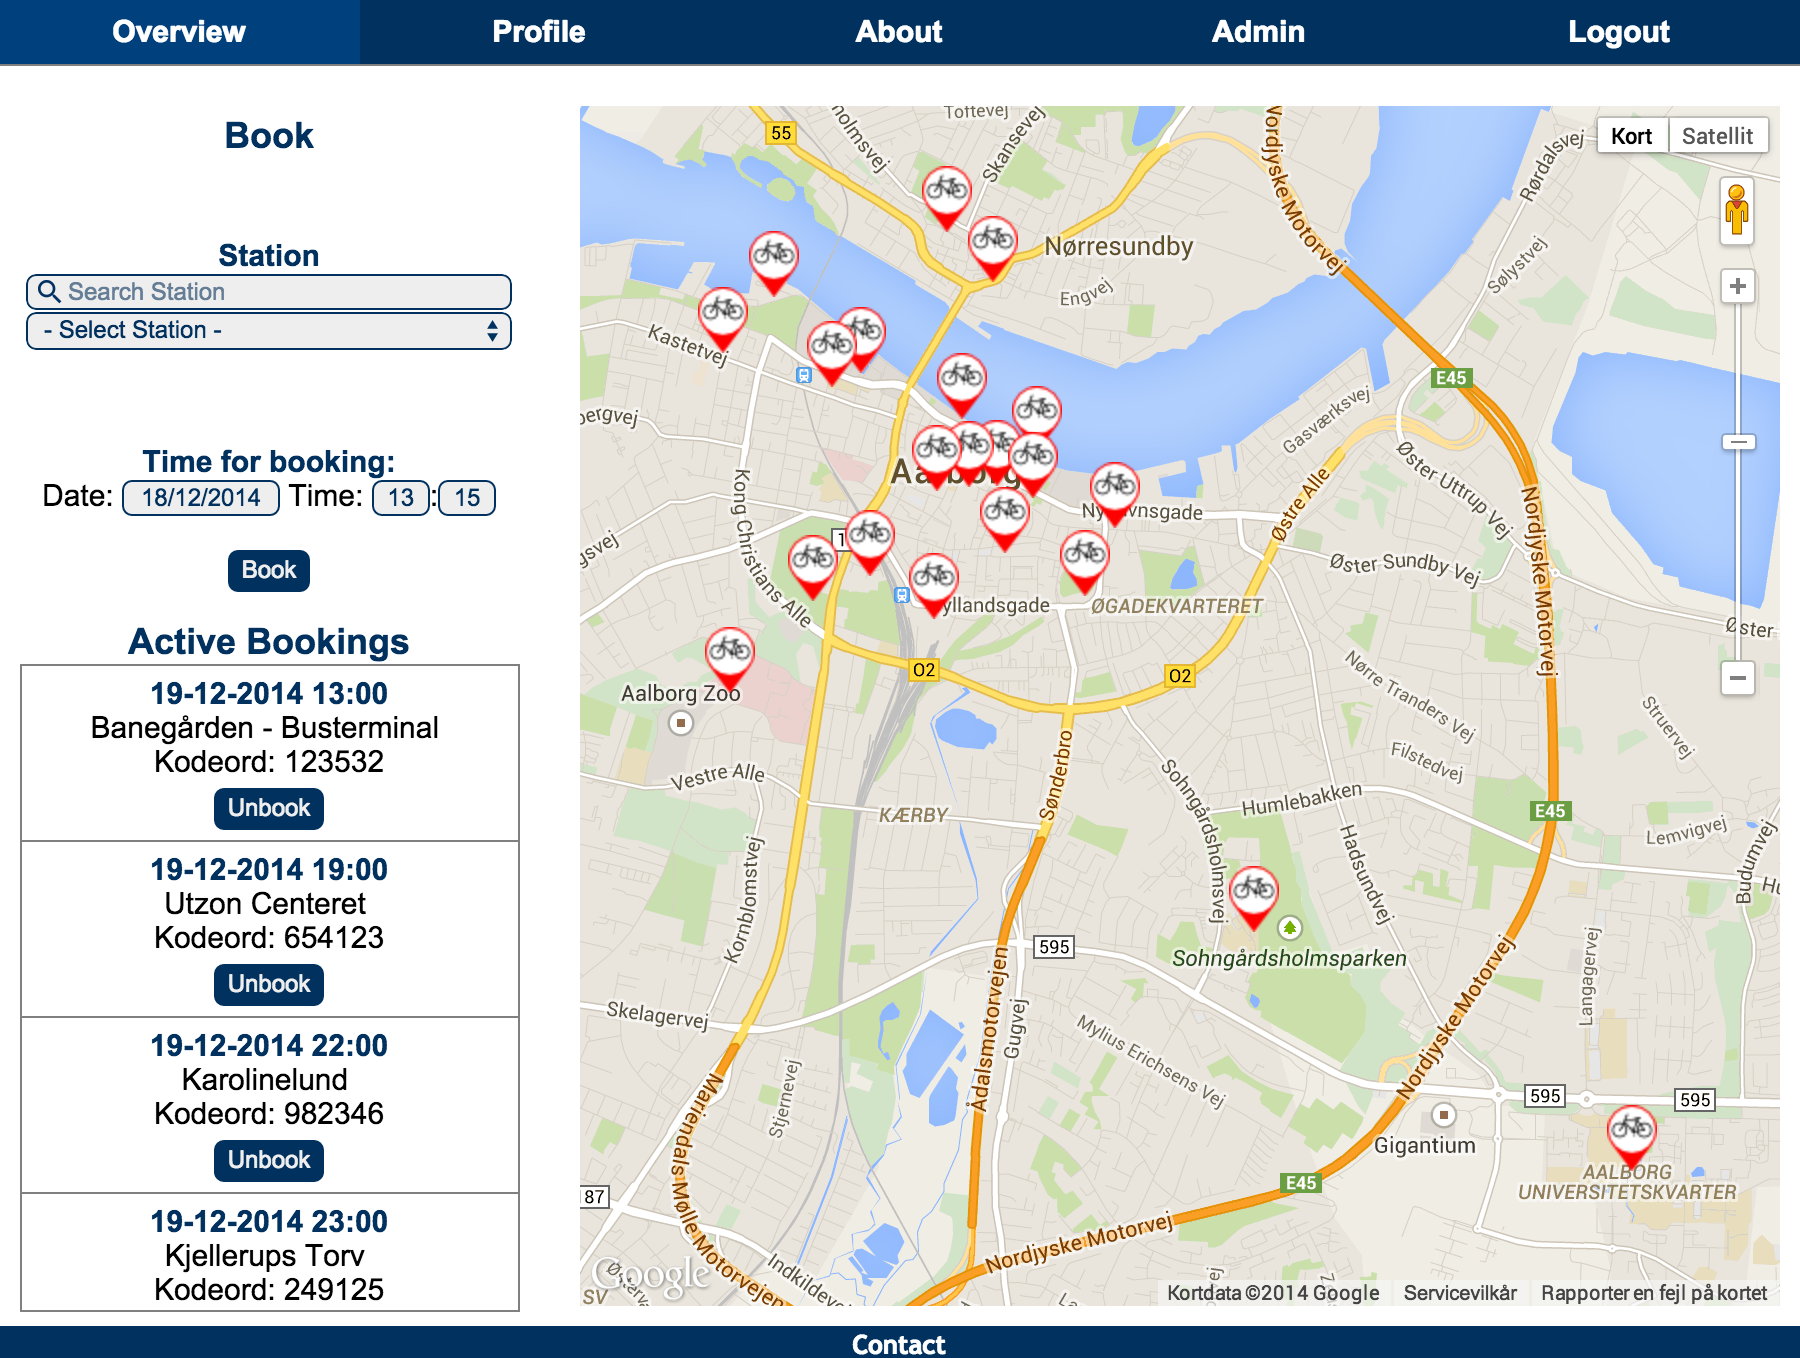
\includegraphics[scale=0.6]{UI/overview}
	\caption{Overview page}\label{fig:UI-overview}
\end{figure}

In this figure we can see that something from the prototype has been changed, mainly the fact that the screen is now only split in two parts, where the map showing station locations covers two thirds, and the bookings/station details cover the last third.
The map in the figure shows a map of Aalborg city with bicycle icons on it representing the station placements.
The right side of the website is used for booking, where users can book a bicycle on a chosen station at a specified time.
Pressing the book button creates a booking at the currently selected station and specified time.
The user can also see a list of bookings he/she currently has, and is able to cancel said bookings by clicking on the unbook button.

In \figref{fig:UI-overview} the header contains five elements, of which the admin element is only shown to admin users and directs the user to the admin section of the site when clicked.
The profile element in the header directs the user to their profile page, where they can change their profile information if so desired, as well as view the history of their usage of the system.


The admin features are created for use by Aalborg Kommune, and they start on the page that can be seen in \figref{fig:UI-admin}.
This page is almost just a map, however, the black dots on the map are used to represent the current position of bicycles.
The header can be used to navigate to the various admin tools, elaborated more in \secref{sec:impAdminTools}.
The only header element that does not direct to another admin site, is the home element, which sends the user to the overview page.
Additionally, if a user tries to access an admin page, via. the url, he will be redirected to the homepage.

\begin{figure}[h]
	\centering
	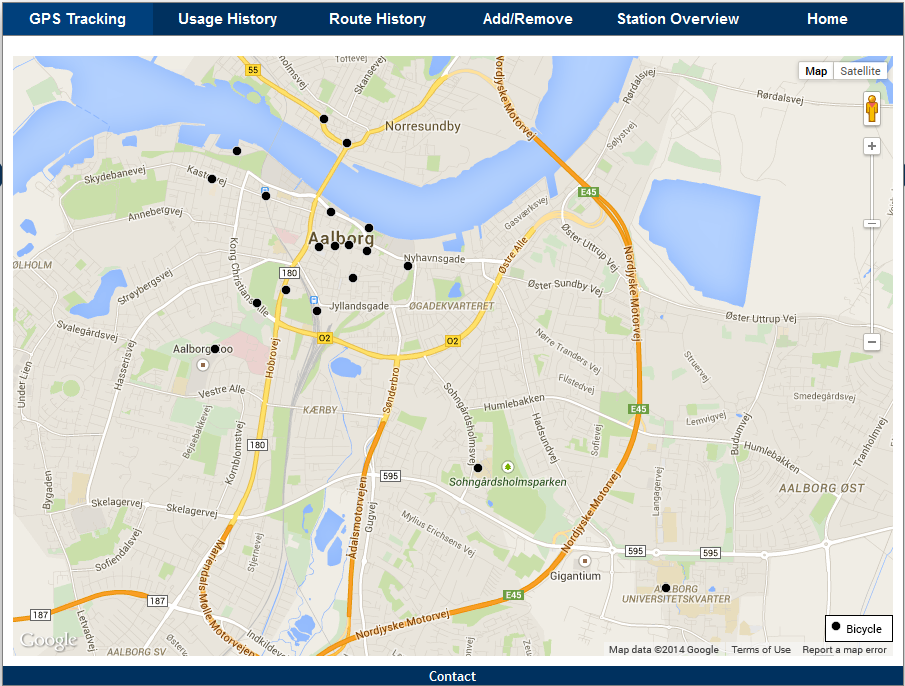
\includegraphics[scale=0.6]{UI/tracking}
	\caption{Admin page}\label{fig:UI-admin}
\end{figure}
